\documentclass{llncs}
\usepackage{graphicx}
\usepackage{hyperref}
\usepackage{listings}
\usepackage{xcolor}
\usepackage[english]{babel}
\usepackage{pdfpages}
\usepackage{tabularx}
\usepackage{booktabs}

\begin{document}
\title{Simple Web Server}


\author{Radu Emilian}
\institute{Universitatea Alexandru Ioan Cuza Iasi, Facultatea de Informatica
\email{mihai.radu@info.uaic.ro}\\
}
\maketitle

\begin{abstract}
Un simplu server web realizat prin socketi.

\keywords{TCP  \and HTTP}
\end{abstract}
\definecolor{mGreen}{rgb}{0,0.6,0}
\definecolor{mGray}{rgb}{0.5,0.5,0.5}
\definecolor{mPurple}{rgb}{0.58,0,0.82}
\definecolor{backgroundColour}{rgb}{0.95,0.95,0.92}
\lstdefinestyle{CStyle}{
    backgroundcolor=\color{backgroundColour},   
    commentstyle=\color{mGreen},
    keywordstyle=\color{magenta},
    numberstyle=\tiny\color{mGray},
    stringstyle=\color{mPurple},
    basicstyle=\footnotesize,
    breakatwhitespace=false,         
    breaklines=true,                 
    captionpos=b,                    
    keepspaces=true,                 
    numbers=left,                    
    numbersep=5pt,                  
    showspaces=false,                
    showstringspaces=false,
    showtabs=false,                  
    tabsize=2,
    language=C
}


\section{Introducere}

\subsection{Cerinta Proiectului}
Realizati un server concurent ce trimite fisiere (.txt sau .html fara scripturi)
din directorul curent catre orice browser se conecteaza la el. Server-ul va trebui sa trimita antete HTTP corecte. 
Nu implementati un client: server-ul va trebui sa interactioneze corect cu orice browser.
 
\subsection{Modul de abordare}
Pentru rezolvarea cerintei se va utiliza drept punct de "start" fisierul servTcpIp.c de pe site-ul cursului, la care se vor face modificari
pentru a accepta conetarea unui client de tipul "browser".\\
Primul pas va fi transformarea serverului initial ce este de tip iterativ intr-un server concurent, pentru a accepta conexiunea mai multor
clienti consecutiv.\\
De asemenea, se va crea fisierul "config.txt" ce contine detalii esentiale pentru functionarea serverului.\\
Fisierele ce vor fi furnizate clientului de catre server vor avea locatia definita in fisierul de configurare specificat anterior si vor avea
extensia .txt, .html, .jpg sau .png (configurabile in fisierul de configurare).

\subsection{Motivatia alegerii proiectului}





\section{Tehnologii Utilizate}
\begin{enumerate}
  \item TCP/IP Concurent
  \item HTTP Protocol
\end{enumerate}
\subsection{TCP/IP Concurent}
A fost utilizat protocolul Transmission Control Protocol (TCP) deoarece
alternativa (UDP) ar fi cauzat pierderi de informatii esentiale
in cadrul transferului de fisiere catre clienti.
Informatia ceruta trebuie sa ajunga in mod exact la clientul ce o cere
iar acest aspect este facilitat doar de protocolul TCP.
\subsection{HTTP Protocol}
Singura modalitate de a transmite fisiere catre un browser este
prin intermediului protocolului HTTP sau
Hypertext Transfer Protocol ce este protocolul utilizat de World Wide Web.





\section{Arhitectura aplicatiei}
\subsection{Diagrama Aplicatiei}
\begin{figure}
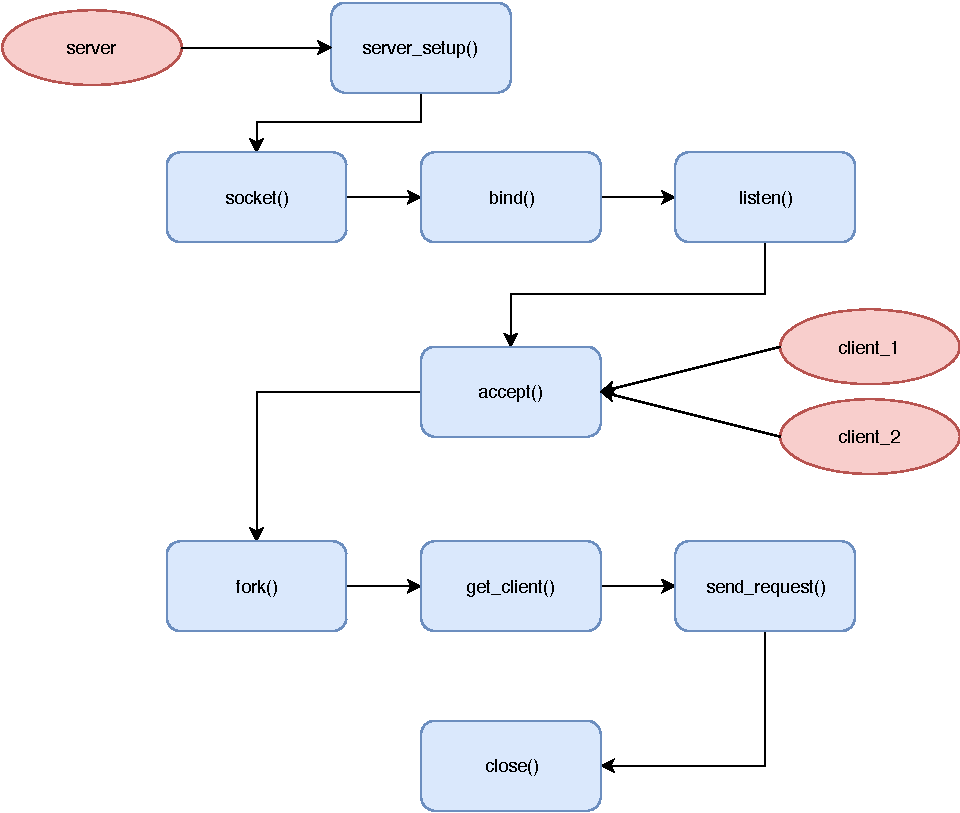
\includegraphics[width=\textwidth]{diagram.pdf}
\end{figure}
\subsection{Concepte implicate}
In cadrul implementarii am modularizat codul, impartindu-l in functii pentru a fi usoara
atat citirea cat si intelegerea programului. Codul este impartit in 4 functii :
\begin{enumerate}
  \item void server\_setup(struct configFile *config);
  \item void get\_client(int client, struct configFile *config);
  \item void send\_request(int client, struct htmlrequest *request, struct configFile *config);
  \item int main(int argc, char **argv)
\end{enumerate}



\section{Detalii de implementare}
\subsection{Cod relevant}
Pentru a retine toate informatiile despre server se va folosi urmatoarea structura:
\begin{lstlisting}[style=CStyle]
struct configFile
{
    int port;
    char address[PATH_DOC];     
    char request[MAXDAT][MAXDAT]; 
    char send[MAXDAT][MAXDAT]; 
    char default_page[MAXDAT];   
};
\end{lstlisting}
Cererea clientului reprezentat de browser va fi salvata in structura:
\begin{lstlisting}[style=CStyle]
struct htmlrequest
{
    char *full, *url, *version, *method;
};
\end{lstlisting}
Acest aspect se va realiza pentru fiecare client in parte, asa ca la finalul cererii se va goli structura prin:
\begin{lstlisting}[style=CStyle]
free(request.full);
free(request.url);
free(request.method);
free(request.version);
\end{lstlisting}
Se va folosi citirea din fisiere destul de frecent:
\begin{lstlisting}[style=CStyle]
    FILE *file_config;
    file_config = fopen(path_file, "r");
    
    if (file_config == NULL)
    {
        perror("[SERVER] Eroare la deschiderea fisierului de configurare: ");
        exit(ERROR);
    }
`
    if (file_config)
    {
        fseek(file_config, 0, SEEK_END);
        length = ftell(file_config);
        buff = malloc(length);
        fseek(file_config, 0, SEEK_SET);
        if (buff)
            fread(buff, 1, length, file_config);
        fclose(file_config);
    }
\end{lstlisting}
Configuratia serverului se va citi in functia server\_config\(\):
\begin{lstlisting}[style=CStyle]
void server_setup(struct configFile *config)

\end{lstlisting}

Dupa ce s-au citit detaliile din fisierul config.txt serverul va realiza bind(), socket() si listen():
\begin{lstlisting}[style=CStyle]
    if ((sd = socket(AF_INET, SOCK_STREAM, 0)) == ERROR)
    {
        perror("[SERVER] Eroare la socket().\n");
        return errno;
    }

    if (bind(sd, (struct sockaddr *)&server, sizeof(struct sockaddr)) == ERROR)
    {
        perror("[SERVER] Eroare la bind().\n");
        return errno;
    }

    if (listen(sd, MAXCL) == ERROR)
    {
        perror("[SERVER] Eroare la listen().\n");
        return errno;
    }
\end{lstlisting}
Clientii vor fi serviti intr-o bucla while() in care se realizeaza fork() pentru a-i servi concurent:
\begin{lstlisting}[style=CStyle]
	if ((pid = fork()) == ERROR)
        {
            perror("[SERVER] Eroare la fork(). \n");
        }
\end{lstlisting}
Functia ce se ocupa de rezolvarea cerintelor clientului este
\begin{lstlisting}[style=CStyle]
void get_client(int client, struct configFile *config)
\end{lstlisting}

Urmatorul pas in servirea clientului dupa ce s-a aflat cererea este trimiterea informatiilor din fisierul cerut:

\begin{lstlisting}[style=CStyle]
void send_request(int client, struct htmlrequest *request, struct configFile *config)
\end{lstlisting}

Rezolvarea cererii se face prin intermediul protocolului HTTP 1.1 (cea mai recenta versiune) cu ajutorul string-urilor:
\begin{lstlisting}[style=CStyle]
    char html[] = "HTTP/1.1 200 OK:\r\n"
            "Content-Type: text/html; charset=UTF-8\r\n\r\n";
\end{lstlisting}

La final, fisierul cerut este transmis prin send()
\begin{lstlisting}[style=CStyle]
send(client, buff, read_bytes, 0);
\end{lstlisting}




\subsection{Scenarii de utilizare}
\begin{enumerate}
  \item Un client doreste sa acceseze pagina de index a serverului.
  \item Un client doreste sa acceseze un fisier specific cu extensia .txt/.html.
  \item Un client doreste sa acceseze o imagine cu extensia .jpg/.png
  \item Un client doreste sa acceseze un fisier care nu exista in root.
\end{enumerate}




\section{Concluzii}
Conform implementarii actuale a serverului, din fisierul de configurare
nu se preiau vectorii request si send, astfel extensiile fisierelor fiind hard-coded.
Pe viitor doresc rezolvarea acestei probleme pentru a putea fi adaugat in fisierul
de configurare oricate extensii - inclusiv .css sau .js.\\
Deoarece mi-am ales acest proiect am reusit sa invat mai multe aspecte ale limbajului
C pe langa  concepte necesare obiectului Retele de Calculatoare, ce ma vor ajuta
atat in crearea/intretinerea unui server pe viitor.






\begin{thebibliography}{8}

\bibitem{ref_url1}
Computer Networks - Faculty of Computer Science, \url{https://profs.info.uaic.ro/~computernetworks/}
\bibitem{ref_book1}
servTCPIt.c, Lenuta Alboaie, adria@infoiasi.ro, (c)2009

\bibitem{ref_book2}
Hypertext Transfer Protocol -- HTTP/1.1, \url{https://www.w3.org/Protocols/rfc2616/rfc2616.html}

\bibitem{ref_book3}
A template to make good README.md, \url{https://gist.github.com/PurpleBooth/109311bb0361f32d87a2}

\bibitem{ref_book3}
C Library - <string.h>, \url{https://www.tutorialspoint.com/c_standard_library/string_h.htm}

\bibitem{ref_book3}
Information for Authors of Springer Computer Science Proceedings, \url{https://www.springer.com/gp/computer-science/lncs/conference-proceedings-guidelines}


\bibitem{ref_book3}
How to read the content of a file to a string in C?, \url{https://stackoverflow.com/questions/174531/how-to-read-the-content-of-a-file-to-a-string-in-c}

\bibitem{ref_book3}
Transmission Control Protocol, \url{https://en.wikipedia.org/wiki/Transmission_Control_Protocol}

\bibitem{ref_book3}
Berkeley sockets, \url{https://en.wikipedia.org/wiki/Berkeley_sockets}




\end{thebibliography}
\end{document}
